\section{Related Work}
\label{sec:related_work}

%-------------------------------------------------------------------------
\noindent\textbf{Medical Universal Models.}
Universal medical image segmentation models aim to address the data heterogeneity across tasks and modalities while learning generalizable feature representations. Early works include multi-dataset learning through label conditioning~\cite{dmitriev2019learning}, organ size constraints~\cite{zhou2019prior}, and pseudo-label co-training~\cite{huang2020multi}. Recent works are placed on sophisticated task encoding strategies. DoDNet~\cite{zhang2021dodnet} pioneered one-hot task vectors with an extension into TransDoDNet~\cite{xie2023learning} using transformer backbones. Advances include CLIP-driven models using semantic encodings~\cite{liu2023clip}, task-specific heads in MultiTalent~\cite{ulrich2023multitalent}, and modality priors in Hermes~\cite{gao2024training}. UniSeg~\cite{ye2023uniseg} introduced learnable task prompts and MedUniseg~\cite{ye2024meduniseg} unified 2D/3D image handling. Despite of substantial efforts, these universal models all require fine-tuning when assessing unseen classes. In contrast, Iris enables the segmentation of unseen classes only through a single reference image-label pair without any model finetuning.

 

\noindent\textbf{SAM-based Interactive Models.}
Segment Anything Model (SAM)~\cite{kirillov2023segment} emerges as a shifting paradigm of interactive segmentation via its prompt-based architecture and large-scale training. SAM's success has inspired a range of medical variants. Major examples include  MedSAM~\cite{ma2024segment} with 1.5M image-mask pairs for 2D segmentation, SAM-Med2D~\cite{cheng2023sam} trained on 4.6M images, and SAM-Med3D~\cite{wang2024sam} extending to volumetric data with 22K 3D images. These efforts all require multiple prompts and interactive refinements, especially for analyzing complex objects in 3D scenarios. This interaction-dependent design becomes a bottleneck in high-throughput scenarios that an automated processing of large-scale datasets is much desired. As comparison, Iris addresses this limitation by defining tasks through context pairs, enabling fully automatic segmentation while maintaining a strong adaptability to new tasks.


\begin{figure*}[t]
\begin{center}
%\framebox[4.0in]{$\;$}
%\fbox{\rule[-.5cm]{0cm}{4cm} \rule[-.5cm]{4cm}{0cm}}
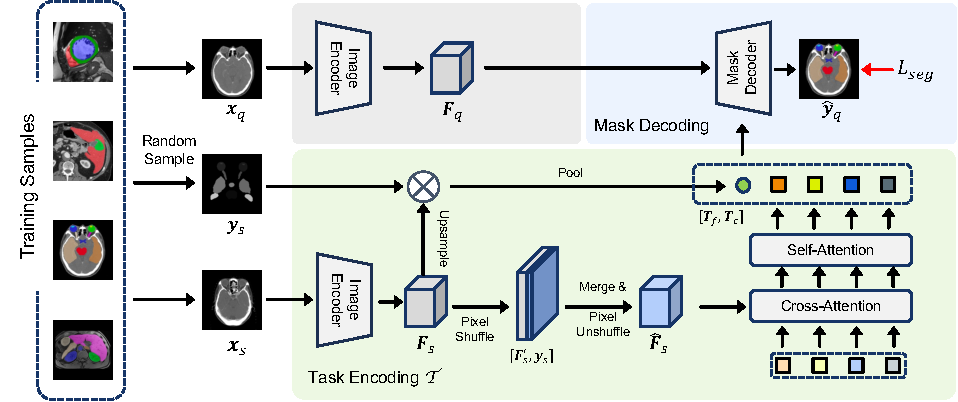
\includegraphics[width=0.9\textwidth]{./fig/framework.pdf}
\end{center}
\vspace{-1em}
\caption{Overview of Iris framework. We design a task encoding module to extract compact task embeddings from reference examples to guide query image segmentation with the mask decoding module, enabling efficient and flexible adaptation to new tasks without finetuning.}
\label{fig:framework}
\vspace{-1em}
\end{figure*}



\noindent\textbf{Visual In-context Learning.} 
In-context learning as introduced by GPT-3~\cite{brown2020language} enables models to handle novel tasks through example-guided inference without a heavy retraining. In the vision community, Painter~\cite{wang2023images} and SegGPT~\cite{wang2023seggpt} pioneered in-context segmentation through a mask image modeling framework. Alternative methods~\cite{liu2023matcher,zhang2023personalize,sun2024vrp} explored SAM-based approaches through cross-image correspondence prompting, but their two-stage pipeline introduces redundant computation and heavily relies on SAM's capabilities, limiting their applicability to 3D medical images. Neuralizer~\cite{czolbe2023neuralizer} develop general tools on diverse neuroimaging tasks, like super-resolution denosing, etc. Recent works introduced specialized architectures for in-context segmentation~\cite{meng2024segic}. For example, UniverSeg~\cite{butoi2023universeg} is designed for in-context medical image segmentation, and Tyche~\cite{rakic2024tyche} incorporated a stochastic inference. While these methods demonstrate promising capability on novel classes, they face two critical limitations. First, they show suboptimal performance compared to task-specific models on the training distribution. Second, they suffer from computational inefficiencies as they can only segment one anatomical class per forward pass, requiring multiple passes for multi-class segmentation. Meanwhile they must re-encode context examples for each query image even when using the same reference examples repeatedly. This becomes particularly problematic in high-throughput scenarios where multiple query images need to be processed. In contrast, Iris shows better performance and efficiency. An appealing design of our context task encoding module is to decouple task definition from inference, enabling the encoding of task from reference pairs into task tokens that can be efficiently reused across any number of query images, meanwhile multi-class segmentation can be done within a single forward pass. 


The selection of appropriate context examples impacts the performance of in-context learning. Current methods~\cite{zhang2023makes} employ image-level retrieval strategies using global image embeddings to find better references. However, this approach faces significant challenges in medical image analysis where each image contains multiple classes including structures like organs, tissues, and lesions. Image-level retrieval inevitably averages features across all structures, leading to a suboptimal reference selection. To address this limitation, Iris introduces an object-level context selection mechanism that enables fine-grained matching of individual classes, focusing on more precise and class-specific reference selection compared to image-level approaches~\cite{zhang2023makes}.
